\section{Ảnh hưởng của BAS-Loss theo từng lớp}
Bảng~\ref{tab:a2-per-class} và Hình~\ref{fig:a2-per-class} cho thấy mức tăng trung bình lớn nhất ở SignSymbol (2,31 điểm phần trăm), Column\_Pole (2,15 điểm phần trăm) và Bicyclist (2,00 điểm phần trăm). Pedestrian tăng 0,98 điểm phần trăm. Ba lớp Column\_Pole, Bicyclist và Pedestrian đều tăng ở cả ba cặp seed. Đây là các lớp nhỏ hoặc có hình dạng mảnh, phù hợp với mục tiêu bổ sung giám sát ở vùng biên dự đoán.

\begin{table}[htbp]
\centering\small
\begin{tabularx}{\linewidth}{@{}Xrrr@{}}
\toprule
Lớp & Đủ loss (\%) & Bỏ BAS-Loss (\%) & Chênh lệch (đpt)\\
\midrule
Bicyclist & $75{,}51 \pm 0{,}63$ & $73{,}51 \pm 1{,}84$ & $+2{,}00 \pm 2{,}10$\\
Building & $90{,}73 \pm 0{,}27$ & $90{,}62 \pm 0{,}10$ & $+0{,}11 \pm 0{,}26$\\
Car & $95{,}09 \pm 0{,}30$ & $95{,}24 \pm 0{,}09$ & $-0{,}16 \pm 0{,}21$\\
Column\_Pole & $45{,}82 \pm 0{,}33$ & $43{,}67 \pm 0{,}76$ & $+2{,}15 \pm 0{,}82$\\
Fence & $70{,}64 \pm 1{,}91$ & $70{,}86 \pm 1{,}91$ & $-0{,}22 \pm 0{,}97$\\
Pedestrian & $74{,}78 \pm 0{,}39$ & $73{,}80 \pm 1{,}27$ & $+0{,}98 \pm 1{,}31$\\
Road & $97{,}13 \pm 0{,}07$ & $97{,}24 \pm 0{,}05$ & $-0{,}11 \pm 0{,}11$\\
Sidewalk & $91{,}59 \pm 0{,}07$ & $91{,}72 \pm 0{,}09$ & $-0{,}13 \pm 0{,}12$\\
SignSymbol & $54{,}28 \pm 2{,}02$ & $51{,}98 \pm 4{,}74$ & $+2{,}31 \pm 2{,}81$\\
Sky & $92{,}61 \pm 0{,}24$ & $92{,}67 \pm 0{,}07$ & $-0{,}06 \pm 0{,}20$\\
Tree & $81{,}17 \pm 0{,}22$ & $80{,}82 \pm 0{,}29$ & $+0{,}35 \pm 0{,}39$\\
\bottomrule
\end{tabularx}
\caption{IoU từng lớp: trung bình và SD qua ba seed. Chênh lệch được ghép theo seed trước khi tổng hợp.}
\label{tab:a2-per-class}
\end{table}


\begin{figure}[htbp]
\centering
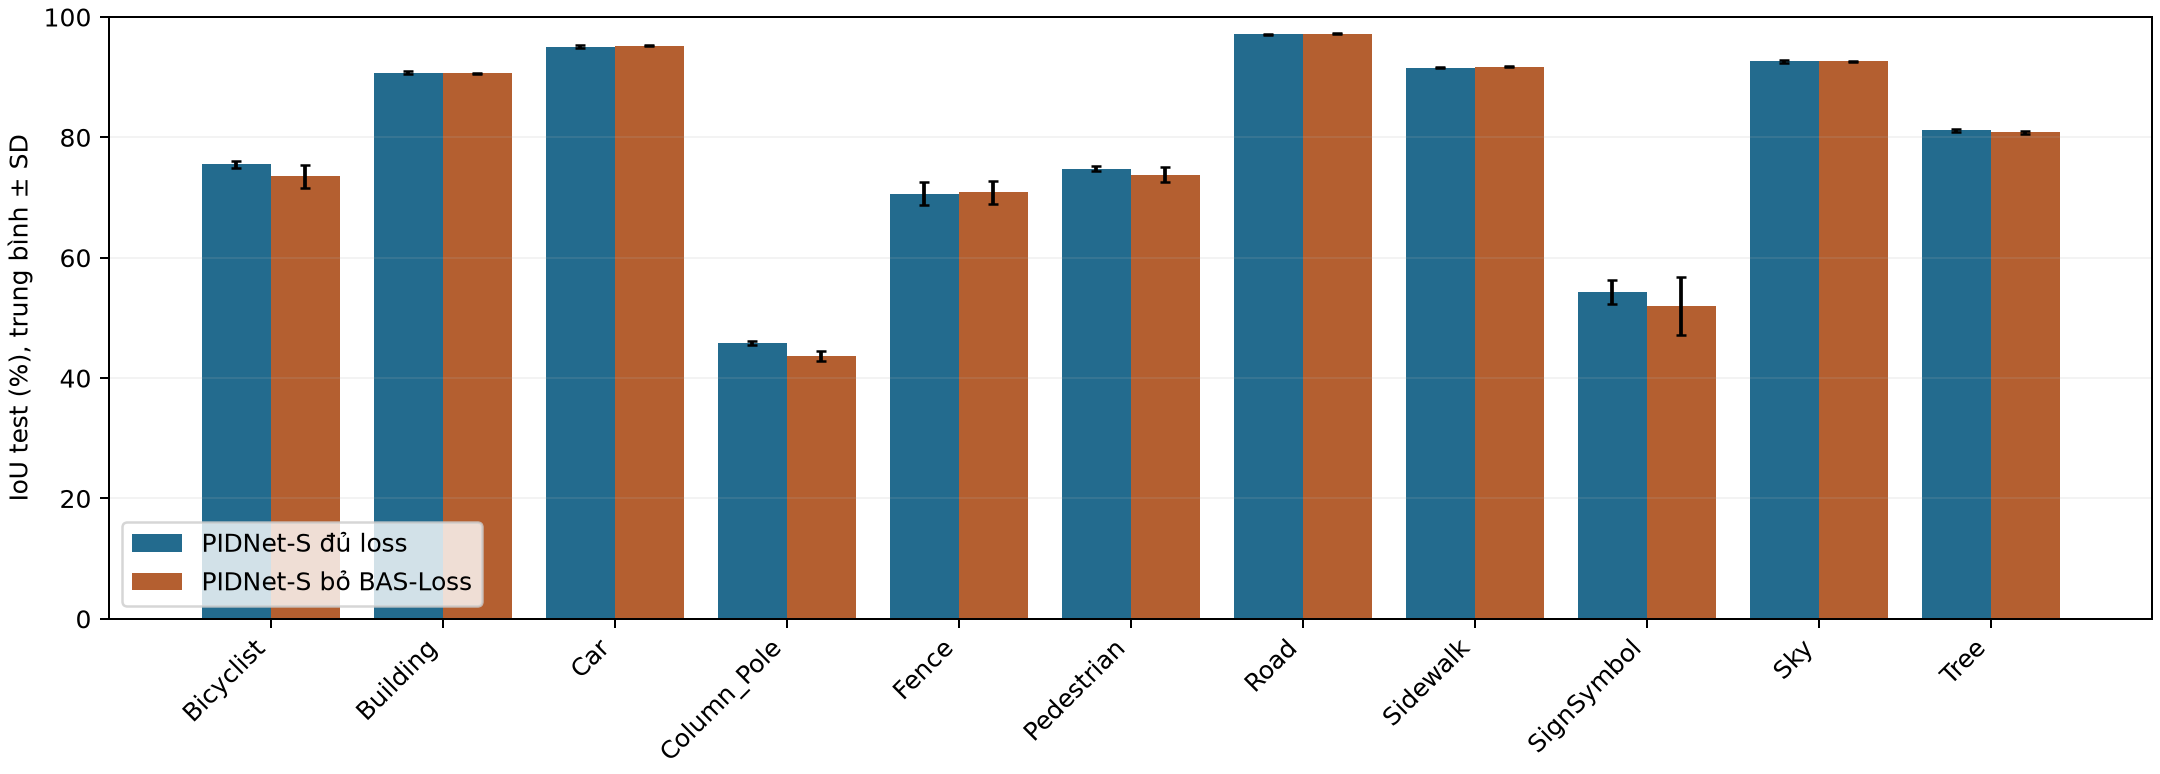
\includegraphics[width=\linewidth]{notebook-evidence/figures/per_class_iou.png}
\caption[IoU test từng lớp qua ba seed.]{IoU test của 11 lớp, lấy trung bình qua ba seed; thanh sai số là độ lệch chuẩn mẫu.}
\label{fig:a2-per-class}
\end{figure}

\Needspace{6\baselineskip}
Mức tăng ở SignSymbol có độ dao động lớn: giảm 0,29 điểm phần trăm ở seed 42, tăng 5,29 ở seed 43 và tăng 1,92 ở seed 44. Trong khi đó, các lớp Car, Fence, Road, Sidewalk và Sky giảm nhẹ về trung bình, với mức giảm dưới 0,22 điểm phần trăm mỗi lớp. Lợi ích mIoU tổng thể vì vậy chủ yếu đến từ một số lớp nhỏ, thay vì tăng đồng đều ở mọi lớp.

Cả hai biến thể vẫn học biên bằng weighted BCE và dùng D trong Light-Bag. Phần bổ sung của bản đủ loss là cross-entropy ngữ nghĩa ở các pixel được boundary head chọn. Kết quả ba cặp seed ủng hộ việc dùng thêm BAS-Loss trong thiết lập này. Phép đo hiện tại là IoU theo lớp, nên chưa tách riêng sai số trong một dải có độ rộng cố định quanh biên.

\subsection{Nhầm lẫn giữa các lớp và ví dụ dự đoán}
Column\_Pole và SignSymbol vẫn là hai lớp khó nhất ở bản đủ loss, với IoU trung bình 45,82\% và 54,28\%. Ở seed 42, bản đủ loss nhận đúng 58,37\% pixel cột, so với 55,58\% của bản bỏ BAS-Loss. Khoảng 20,82\% pixel cột vẫn bị gán thành Building. Với SignSymbol, 24,07\% pixel bị gán thành Building ở bản đủ loss. Các cột và biển báo nhỏ nằm trước tòa nhà vì vậy còn dễ bị lẫn với nền phía sau.

\begin{figure}[htbp]
\centering
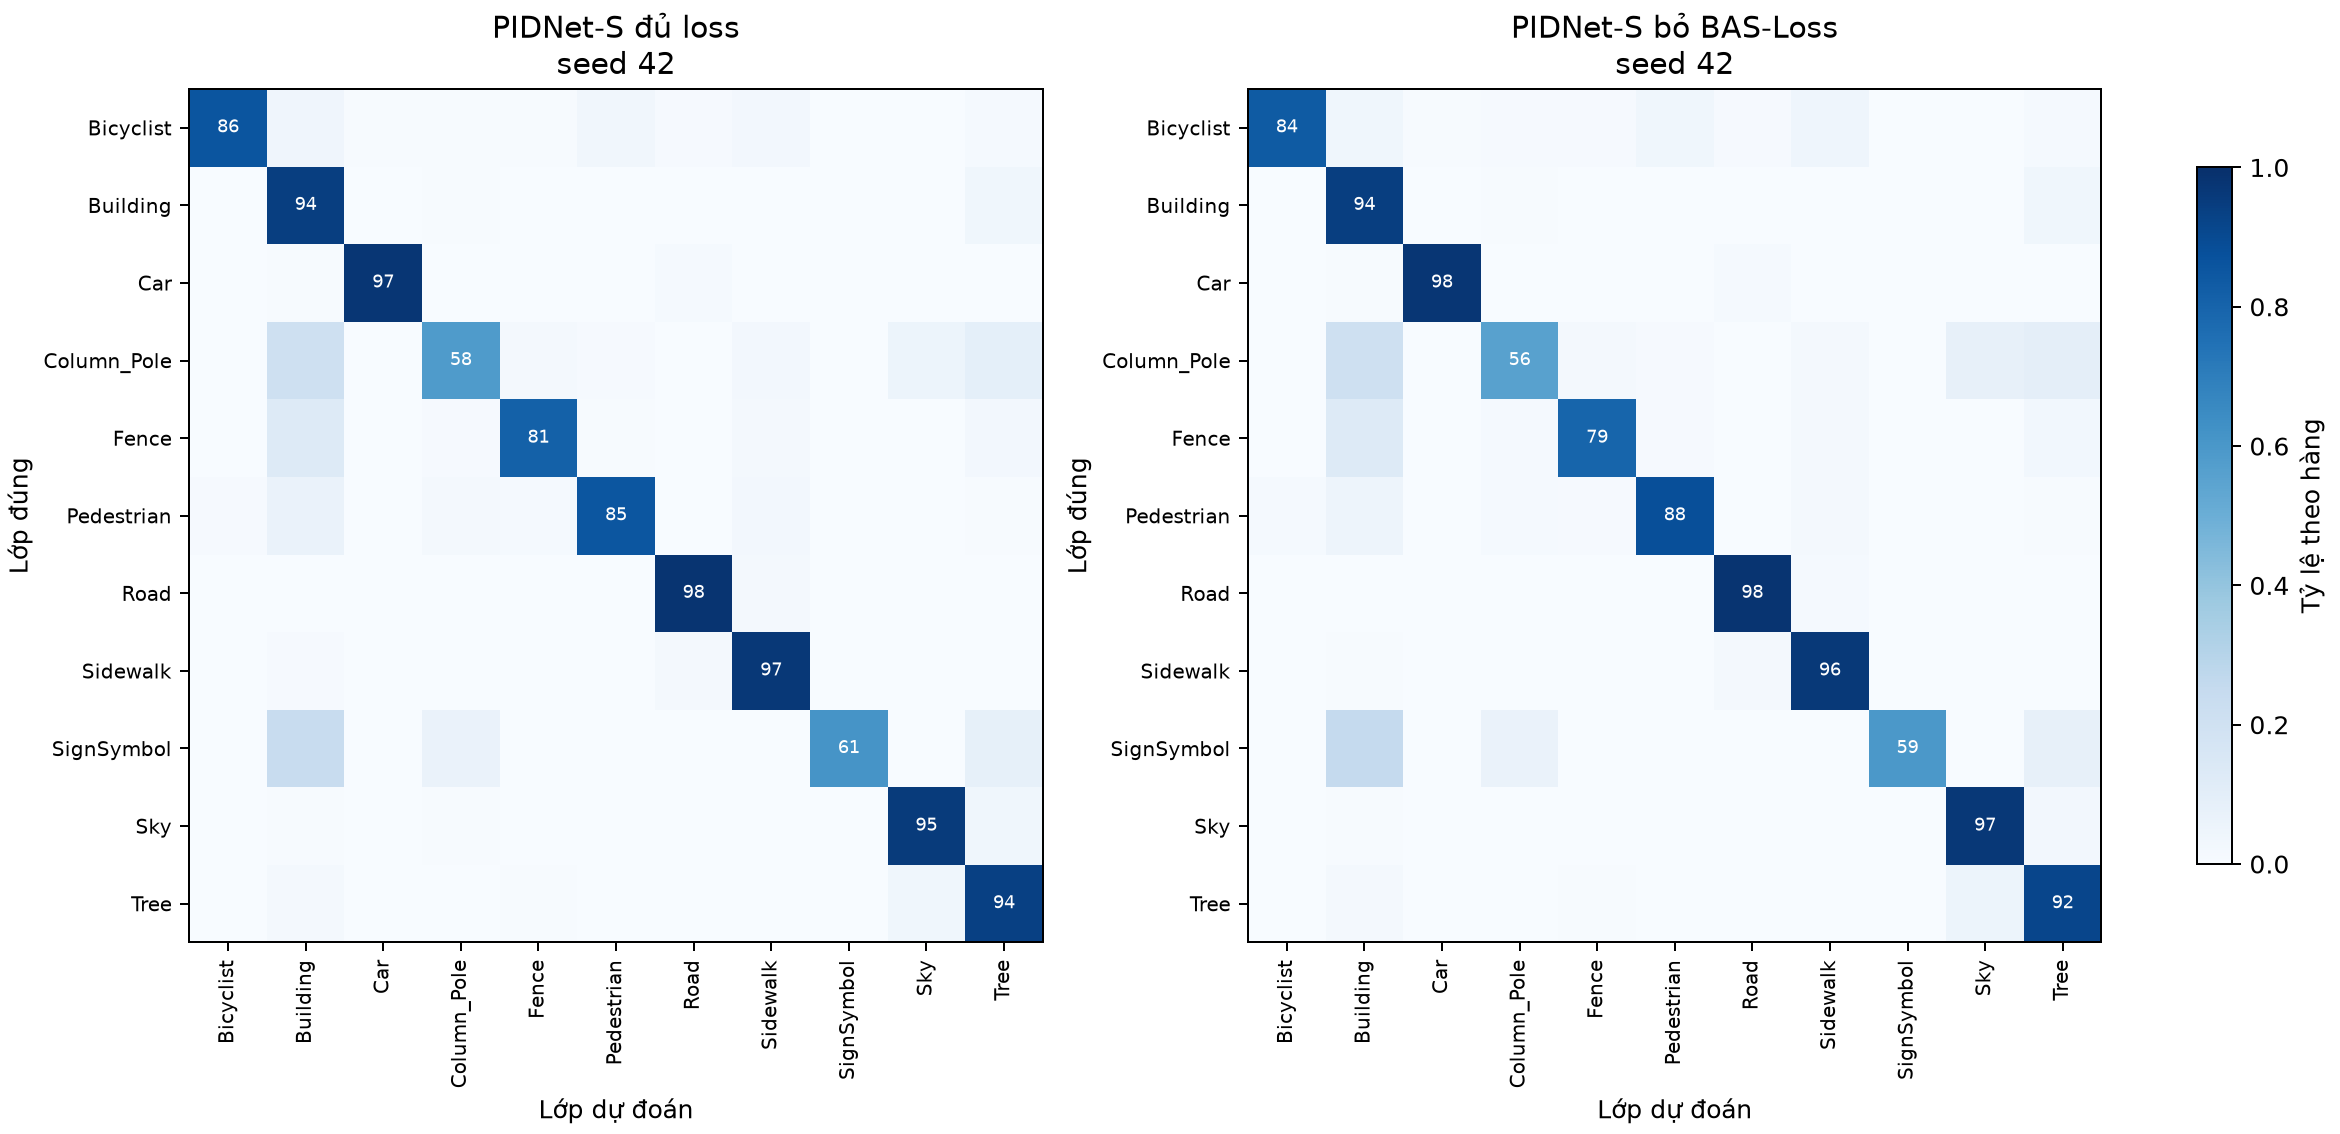
\includegraphics[width=\linewidth]{notebook-evidence/figures/test_confusion.png}
\caption[Confusion matrix test của hai checkpoint seed 42.]{Confusion matrix trên test của hai checkpoint seed 42, chuẩn hóa theo hàng. Đường chéo là tỷ lệ pixel của mỗi lớp được nhận đúng; các con số trên đường chéo tính bằng phần trăm.}
\label{fig:a2-confusion}
\end{figure}

Hình~\ref{fig:a2-examples} dùng ba ảnh tại các vị trí cố định 0, 77 và 155 trong danh sách test, cùng checkpoint seed 42. Hai bản đều nhận ra các vùng lớn như mặt đường, tòa nhà và xe. Các cành cây mảnh còn bị gộp thành những vùng Tree đặc hơn so với nhãn đúng. Sự khác biệt giữa hai bản khó thấy khi chỉ nhìn các vùng lớn; bảng IoU theo lớp và confusion matrix bổ sung thông tin cho các ví dụ này.

\begin{figure}[H]
\centering
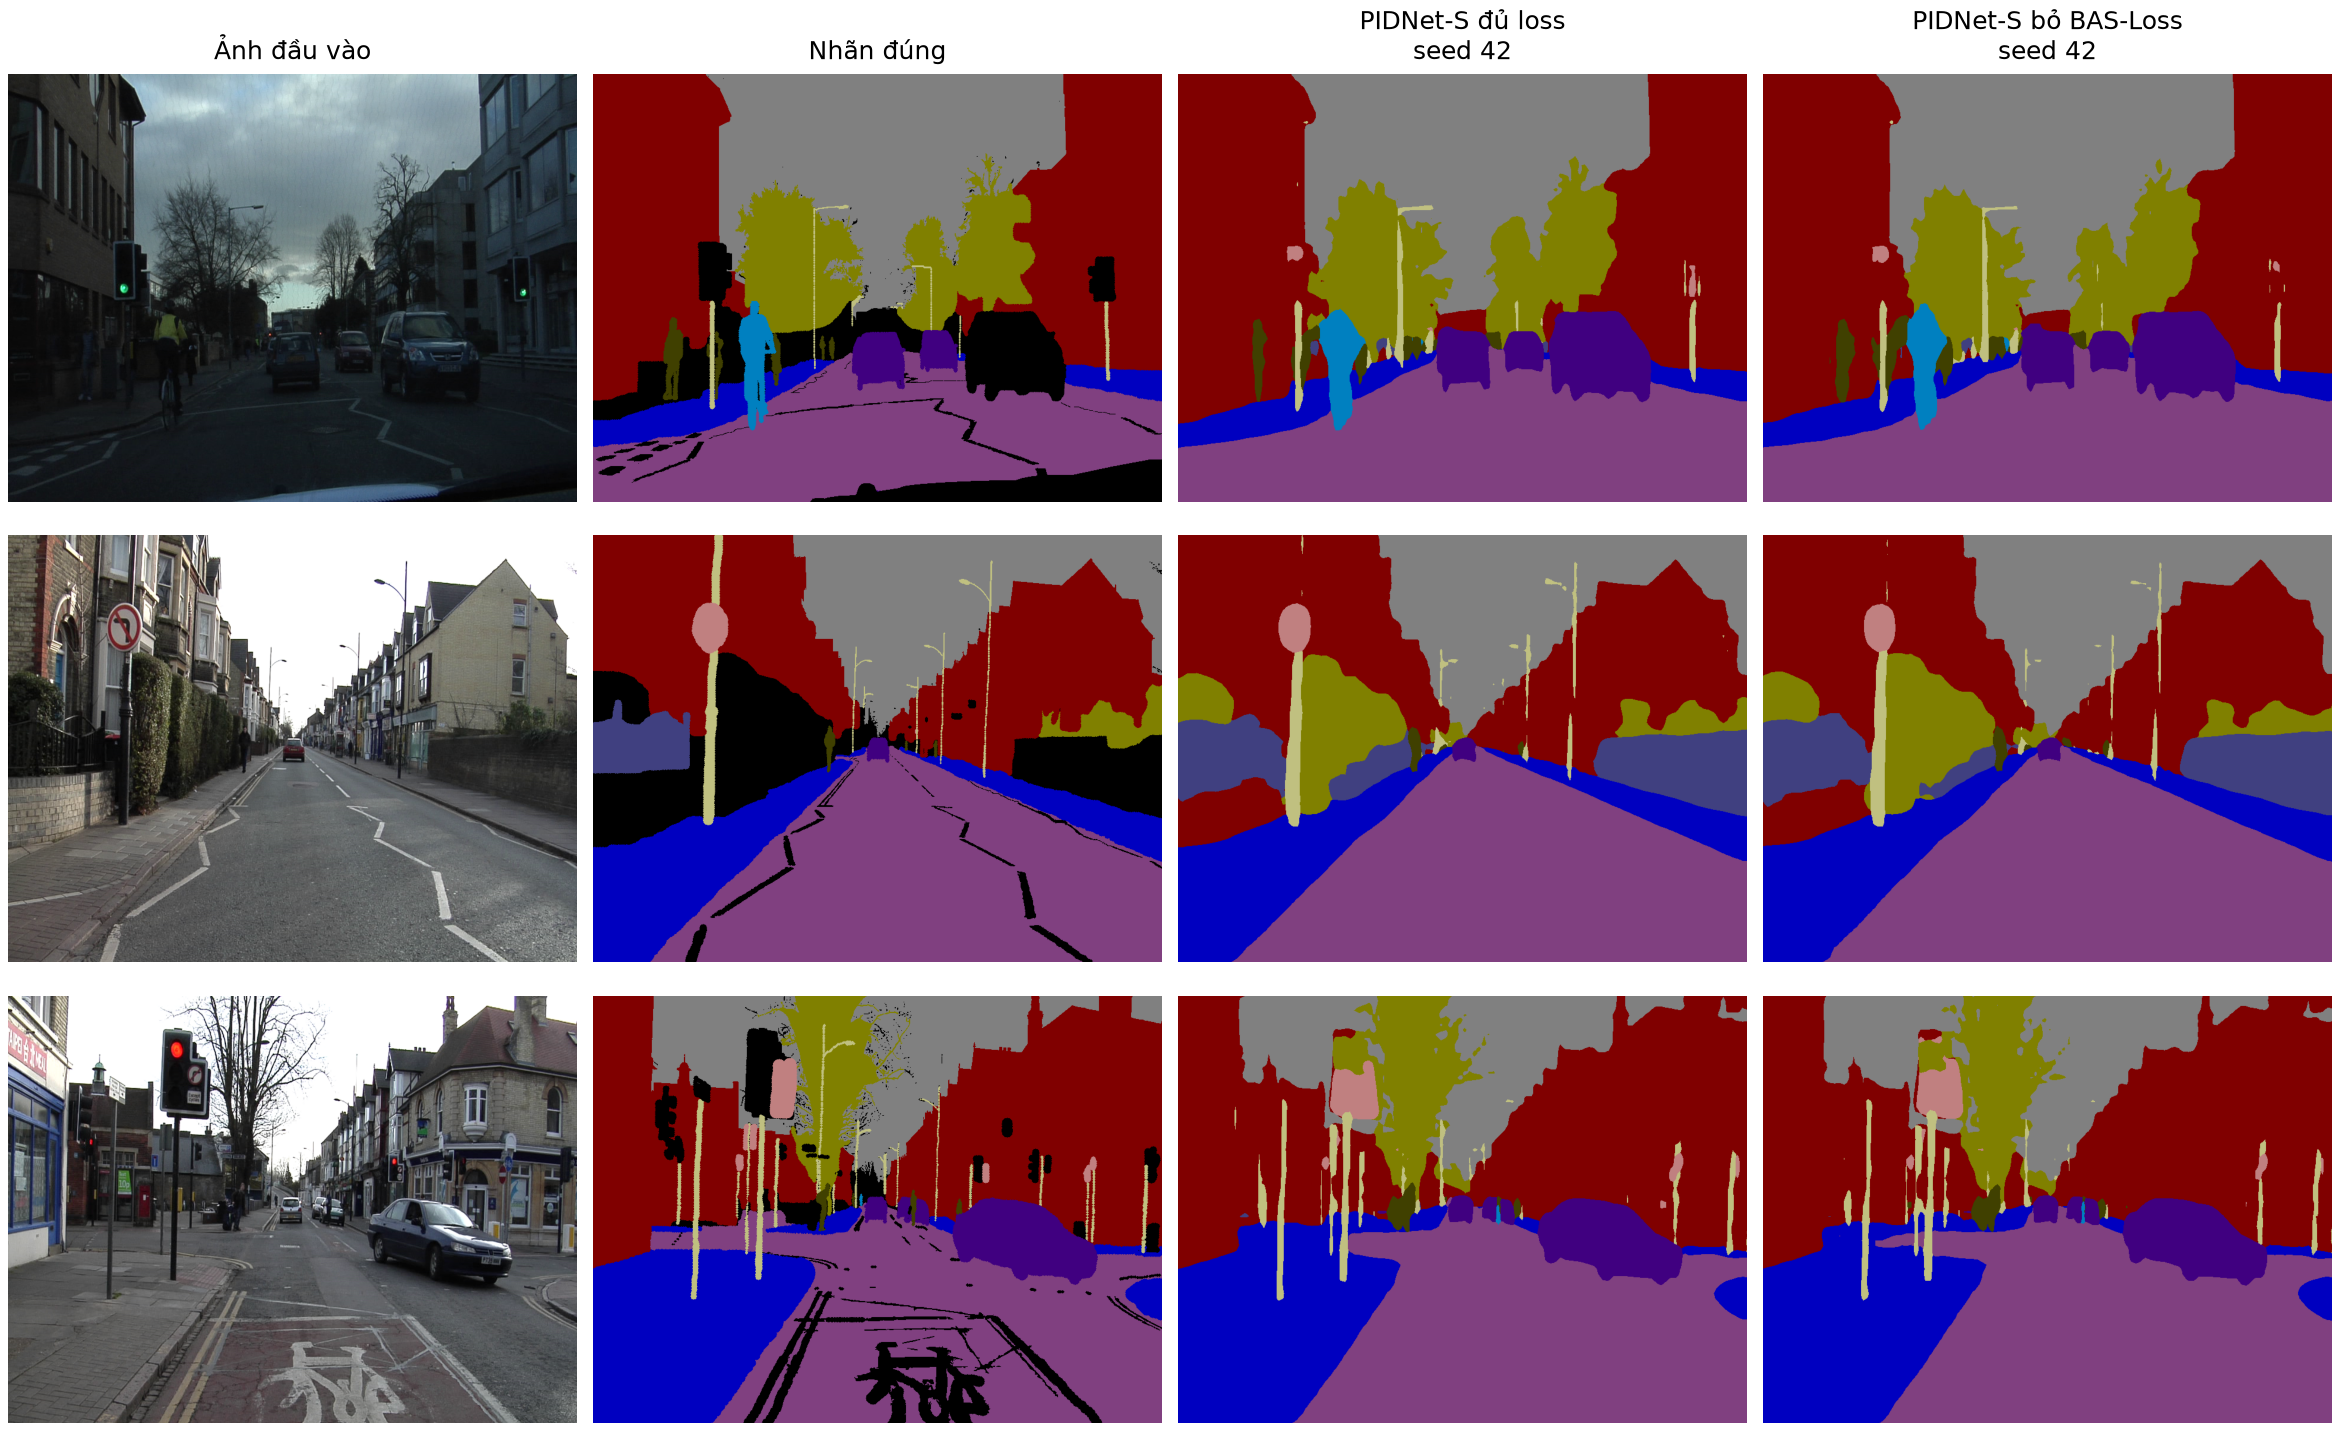
\includegraphics[width=\linewidth,height=0.72\textheight,keepaspectratio]{notebook-evidence/figures/qualitative_comparison_report.png}
\caption[Ba ảnh test và dự đoán của hai biến thể ở seed 42.]{Ba ảnh CamVid test, nhãn đúng và dự đoán của hai biến thể ở seed 42. Màu theo Bảng~\ref{tab:camvid-labels}; màu đen trong nhãn đúng là vùng bỏ qua.}
\label{fig:a2-examples}
\end{figure}
